\documentclass{swfcthesis}

\addbibresource{thesis.bib}    % 参照教程自己去写一个.bib文件

\begin{document}

\Title{操作系统探索}
\Author{尹志成}
\Advisor{王晓林}
\AdvisorTitle{讲师}
\AdvisorInfo{王晓林,男,49 岁,硕士,讲师,毕业于英国格林尼治大学,分布式计算系统专业。
  现任西南林业大学计信学院教师。执教 Linux、操作系统、网络技术等方面的课程,有丰富的 Linux 教学和系统管理经验。}
\Month{六}
\Year{二〇一八}
\Subject{计算机科学与技术专业}    %专业名称(比如 计算机科学与技术专业)
\Abstract{操作系统最初的诞生是为了搭配进行简单繁重的数字运算机,但随着时代的演进,
  计算机不仅作为处理各种运算的机器,其附加价值也越来越被人们看重,跟随着计算机的发展,
  操作系统的使命也在一代代的改变,(约两百字)}
\Keywords{操作系统}
\Acknowledgments{感谢,}
\enTitle{Operating system exploration}
\enAuthor{Zach Yin}
\enAbstract{英文摘要}
\enKeywords{Operate System}

%%% 下面六行不要动!
\makepreliminarypages% 封面
\frontmatter          
\tableofcontents     % 目录
\listoffigures       % 插图目录
\listoftables        % 表格目录
\mainmatter

\chapter{绪论}
在数字时代,操作系统的重要性不言而喻,它作为计算机软硬件之间的桥梁,存在于日常生活的每一个角落,
而研究一个只有庞大的公司聚集成百上千的高级工程师才能完成的操作系统对于学生而言是一个几乎不可能完成的挑战,
但是克服难关是锻炼技术的必经之路\cite{30_os},所以研究并完成一个基本满足日常功能需求的操作系统作为此次的目标,
并以此为跳板对操作系统进行更深一步的探究。

\chapter{思路}

此次的思路由四部分组成:\\
\hspace*{1.5cm}1、操作系统探究 \\
\hspace*{1.5cm}2、空白操作系统的启动 \\
\hspace*{1.5cm}3、编写操作系统内核 \\
\hspace*{1.5cm}4、实现对外兼容及安全防护

\section{操作系统探究}
从历史上计算机操作系统的发展联系到人们的日常生活,寻求符合操作系统发展且适应用户使用的特征要素。

\section{空白操作系统的启动}
利用汇编语言及操作系统相关知识探究操作系统如何从电气设备到软件代码的衔接

\section{丰富操作系统内容}
从内存管理,输入输出,多进程,分时四个模块丰富操作系统的内容

\section{实现对外接口及安全防护}
从接口设计及安全防护的角度完善操作系统

\chapter{操作系统探索}

\section{操作系统的诞生}

\subsection{第一代:真空管}

操作系统最初出现的场景是一个工程师小组设计、建造一台机器,之后使用机器语言编写程序并通过将上千根电缆接到插线板上连接成电路,
控制机器的基本功能,进而操作机器运算诸如制作正弦、余弦、对数表或计算炮弹弹道的简单数学运算。

这里的人工拔插电缆就充当着操作系统的角色——根据程序直接操作硬件使其运算得出结果。

\subsection{第二代:晶体管}

在晶体管发明后,计算机可靠程度大大增加,计算机开始被一些公司、政府部门或大学使用。

改进后出现了操作系统的载体,卡片和较后期磁带打孔纸带。

由于打孔纸带是分次读入,一次只能读入一个的作业,出现了批处理系统如图~\ref{fig:btss}~\ref{tanenbaum2009modern}: 

\begin{figure}[h]
  \centering
  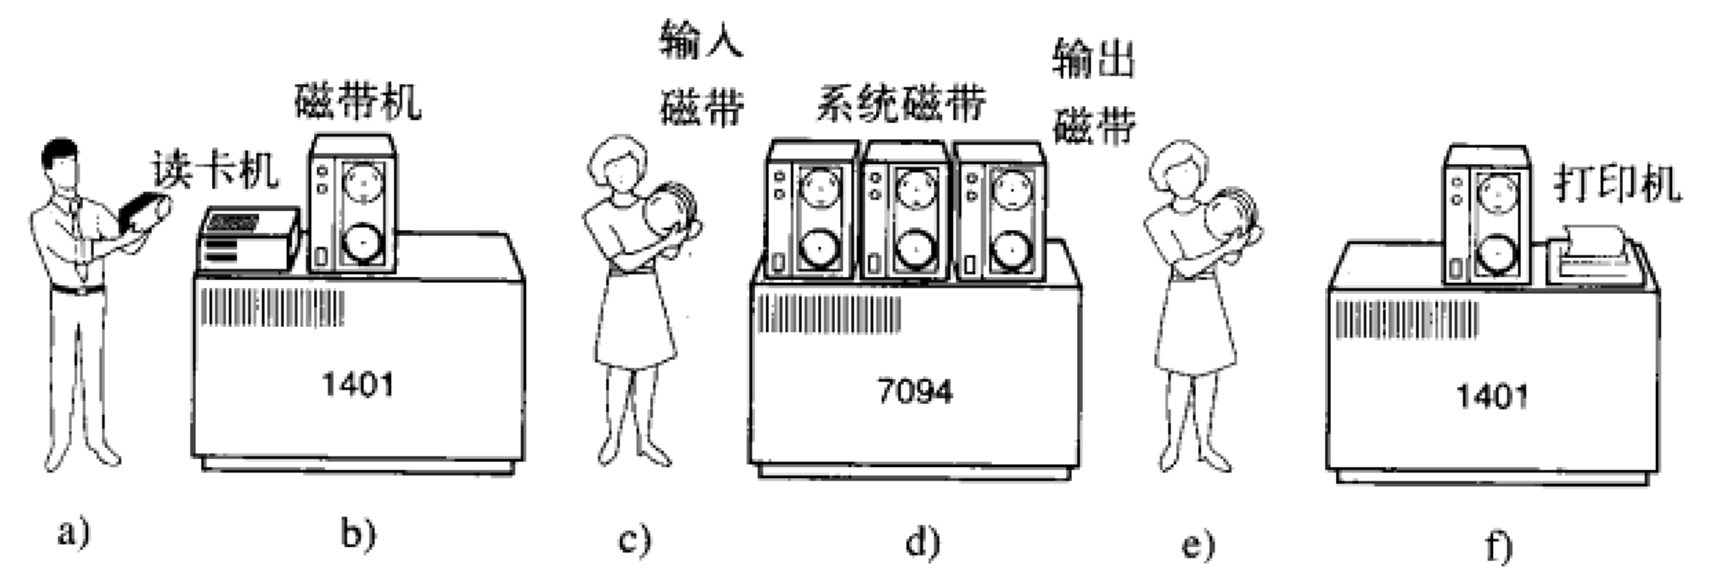
\includegraphics[width=.8\textwidth]{fig/btss.png}
  \caption{批处理系统}
  \label{fig:btss}
\end{figure}

\begin{description}
\item[a.]程序员将打孔纸带拿到1401机\footnote{IBM 1401:数据处理计算机\cite{ibm1401}}
\item[b.]1401机将批处理作业读到磁带上
\item[c.]操作员将输入磁带送至7094机\footnote{IBM 7094:专为大型科学计算而设计,具有出色的性价比和扩展的计算能力\cite{ibm7094}}
\item[d.]7094机进行计算
\item[e.]操作员将输出磁带送到1401机
\item[f.]1401机打印输出
\end{description}

在这里,操作系统的工作已经由完全的人工转换到一部分人工操作交由机器完成,工作效率较之前大大提高,
并且,由于加入了磁带,计算机完成的工作也将及时得到保存。

操作系统的工作已经开始有一定的流程化了。

\subsection{第三代:集成电路}

采用集成电路的第三代计算机较分立晶体管的第二代计算机在性能/价格比上有了很大的提高,

第三代操作系统也加入了多道程序设计和分时系统。

多道程序设计主要目的是解决CPU因等待磁带或其他I/O操作而暂停工作,多道程序设计可以使CPU在程序a的I/O操作时运行程序b。

分时系统解决的主要问题是多用户使用分离的终端,却操作同一台计算机。

\subsection{第四代:个人计算机}

大规模集成电路进一步减小了计算机的大小

\subsection{第五代:移动计算机}

\section{操作系统的规范化}

\chapter{空白操作系统的启动}

\section{操作系统启动流程}

按下电源键之后启动计算机,启动过程分为3个阶段\cite{hbt}:
\begin{center}BIOS -> MBR -> 操作系统\end{center}

\begin{enumerate}
\item 在BIOS完成POST(硬件自检,Power-On Self Test)并根据启动顺序(Boot Sequence)
  来选择启动设备。本系统是从U盘启动。
\item 计算机读取该设备的MBR(第一个扇区,最前面的512个字节,见图~\ref{fig:mbr}),
  并运行其中的启动程序IPL(Initial Program Loader),将ZOS加载入内存。本部分的实现
  代码,参见程序~\ref{sec:ipl09.nas};
\item 控制权转交给操作系统后,Kernel开始运行,操作系统启动成功。
\end{enumerate}

\begin{figure}
  \centering
  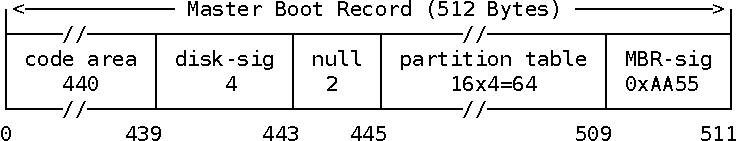
\includegraphics[width=1\textwidth]{fig/mbr.pdf}
  \caption{MBR}
  \label{fig:mbr}
\end{figure}

\section{制作MBR}

MBR负责指出操作系统的位置,主分区第一个扇区的物理位置(柱面、磁头、扇区号等等)

\begin{listing}[H]
  \inputminted[tabsize=2, firstline=6, lastline=6,
  linenos=true]{nasm}{../ZOS/src/kernel/ipl09.nas}
  \inputminted[tabsize=2, firstline=12, lastline=29,
  linenos=true]{nasm}{../ZOS/src/kernel/ipl09.nas}
  \caption{Example of a listing.}
  \label{lst:example}
\end{listing}

\inputminted[tabsize=2, firstline=43, lastline=45,
linenos=true]{nasm}{../ZOS/src/kernel/ipl09.nas}

\inputminted[tabsize=2, firstline=76, lastline=88,
linenos=true]{nasm}{../ZOS/src/kernel/ipl09.nas}

\begin{listing}[H]
  \inputminted[tabsize=2, firstline=125, lastline=147,
  linenos=true]{nasm}{../ZOS/src/kernel/ipl09.nas}
\end{listing}

\section{制作空白操作系统}

首个操作系统为测试操作,目的是测试MBR可以成功启动操作系统

\begin{minted}{nasm}
  fin:
      HLT
      JMP fin
\end{minted}

\begin{listing}[H]
  fin:
  HLT
  JMP fin
\end{listing}

\chapter{编写操作系统内核}

从内存管理,输入输出,多进程,分时四个模块丰富操作系统的内容

\section{内存管理}

内存 (RAM) 是计算机中不可或缺的重要硬件,所有程序的运行都是在内存中进行的,
而CPU访问硬盘数据也必须先经过内存交换才得以实现,内存在加速CPU访问硬盘居功至伟。
由内存的重要性可知内存管理在操作系统中也非常重要。	

内存管理设计的主要目的是快速并且高效的分配内存空间,并在适当的时间释放并回收内存空间。
根据内存管理的设计目的,内存管理的数据结构如下:

\inputminted[tabsize=2, firstline=137, lastline=143,
linenos=true]{c}{../ZOS/src/kernel/bootpack.h}

\begin{description}
\item[frees:]可用信息数目
\item[maxfrees:]用于观察可用状况:frees的最大值
\item[lostsize:]释放失败的内存的大小总和
\item[losts:]释放失败次数
\end{description}

经过内存初始化和释放所有内存空间后,内存管理正常运行。

\subsection{内存分配}

\begin{listing}[H]
  \inputminted[tabsize=2, firstline=68, lastline=80,
  linenos=true]{c}{../ZOS/src/kernel/memory.c}
\end{listing}

\subsection{内存释放}

为保证磁盘空闲空间尽可能不呈现碎片化,内存释放主要分为三种情况:

\begin{description}
\item[前端空闲:]释放内存的相连前端是空闲内存或释放内存相连两端都是空闲内存
\item[后端可用:]释放内存的相连后端是空闲空间
\item[前端后端均不可用:]挪动空闲空间以合并
\end{description}

已知:待释放的空间的开始地址和空间大小

\newpage

前端空闲如图\ref{fig:mem0}和图\ref{fig:mem1}所示: 

\begin{figure}[h]
  \centering
  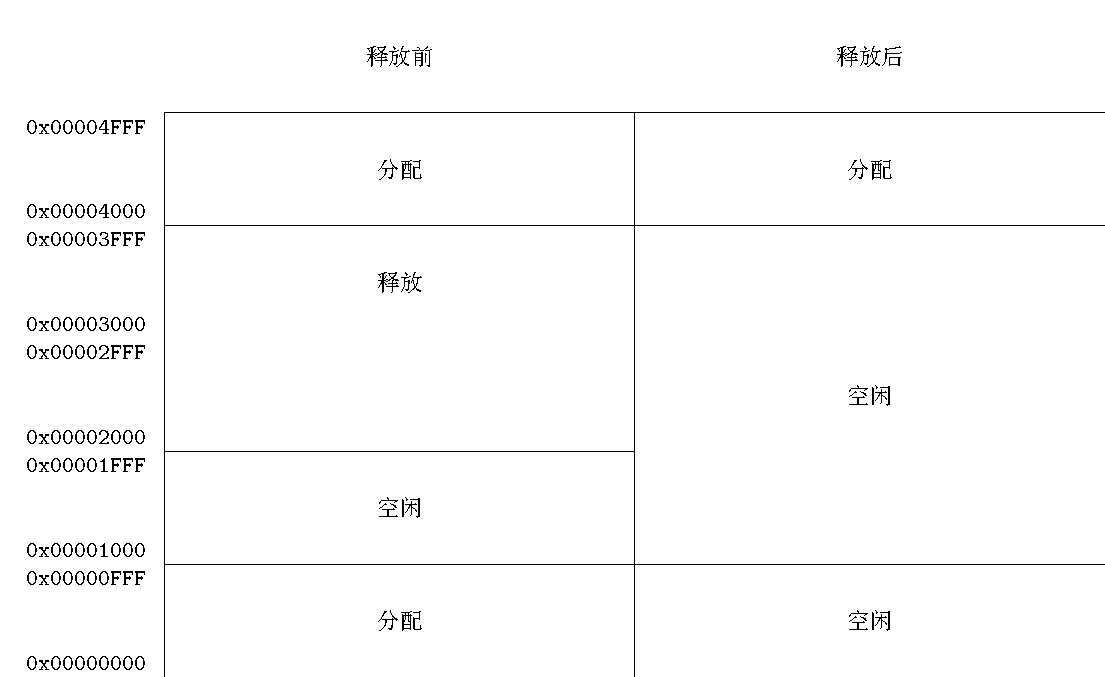
\includegraphics[width=.7\textwidth]{fig/mem0.pdf}
  \caption{前端空闲}
  \label{fig:mem0}
\end{figure}

\begin{figure}[h]
  \centering
x  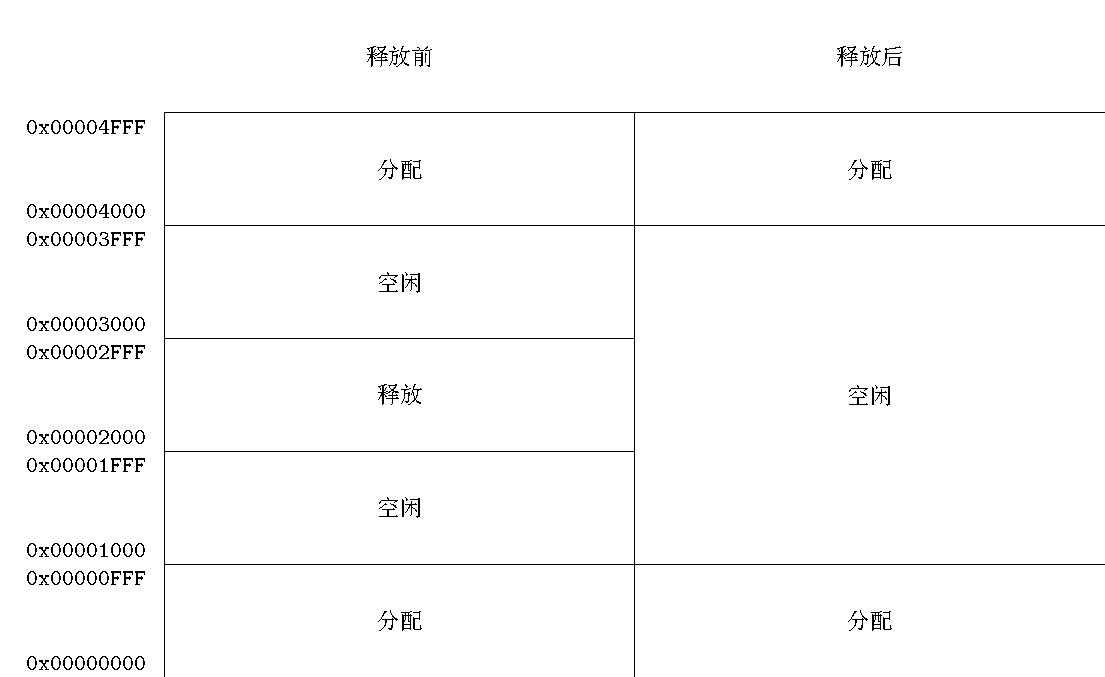
\includegraphics[width=.7\textwidth]{fig/mem1.pdf}
  \caption{前端可用,且后端空闲}
  \label{fig:mem1}
\end{figure}

实现如下:

\begin{listing}[H]
  \inputminted[tabsize=2, firstline=98, lastline=116,
  linenos=true]{c}{../ZOS/src/kernel/memory.c}
\end{listing}

后端空闲:

\begin{figure}[h]
  \centering
  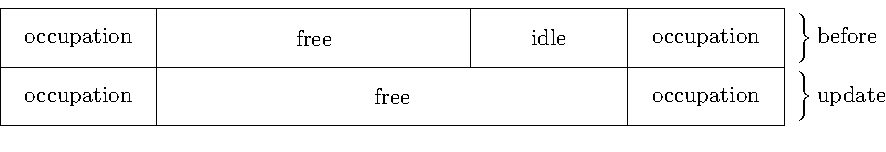
\includegraphics[width=.7\textwidth]{fig/mem2.pdf}
  \caption{后端空闲}
  \label{fig:mem3}
\end{figure}

实现如下:

\begin{listing}[H]
  \inputminted[tabsize=2, firstline=118, lastline=127,
  linenos=true]{c}{../ZOS/src/kernel/memory.c}
\end{listing}

前端后端均被占用:

\begin{figure}[h]
  \centering
  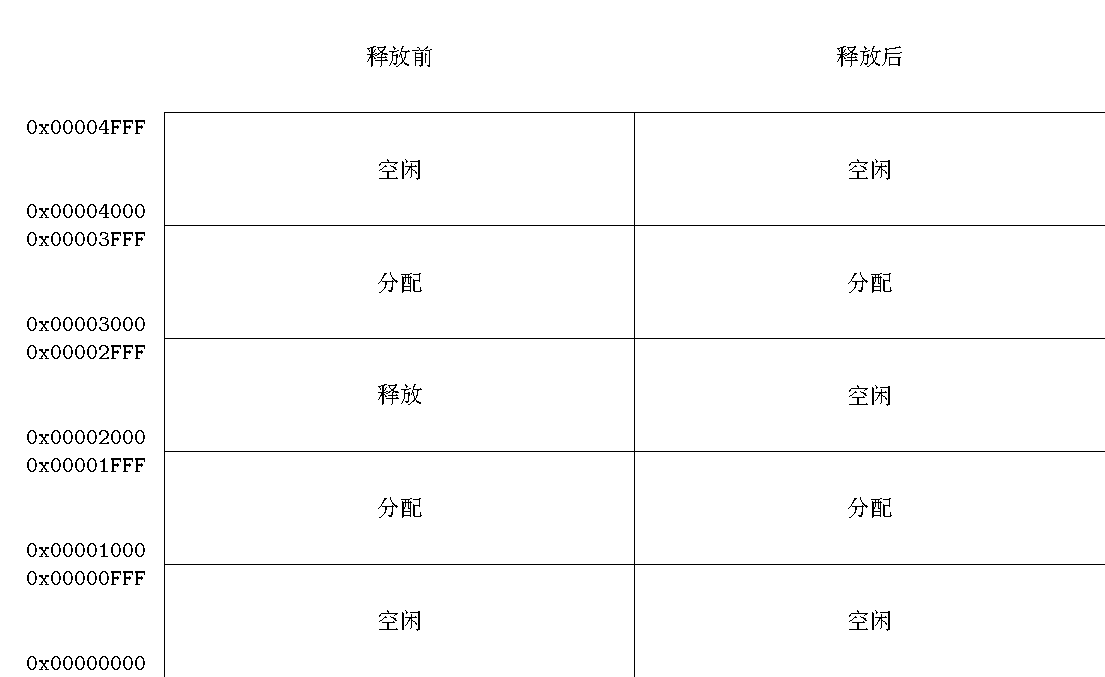
\includegraphics[width=.7\textwidth]{fig/mem3.pdf}
  \caption{前端后端均被占用}
  \label{fig:mem4}
\end{figure}

实现如下:

\begin{listing}[H]
  \inputminted[tabsize=2, firstline=128, lastline=141,
  linenos=true]{c}{../ZOS/src/kernel/memory.c}
\end{listing}

\section{输入输出}

输入作为人与计算机之间最基本的交互方式,其中键盘和鼠标作为标准输入设备。

\subsection{键盘输入}

\begin{listing}[H]
  \inputminted[tabsize=2, firstline=162, lastline=170,
  linenos=true]{c}{../ZOS/src/kernel/bootpack.c}
\end{listing}

\subsection{鼠标输入}

\begin{listing}[H]
  \inputminted[tabsize=2, firstline=247, lastline=265,
  linenos=true]{c}{../ZOS/src/kernel/bootpack.c}
  \inputminted[tabsize=2, firstline=329, lastline=338,
  linenos=true]{c}{../ZOS/src/kernel/bootpack.c}
\end{listing}

\subsection{标准输出}


\section{多道程序系统}

现代的计算机已经不仅仅作为数字计算的工具,而进入大众生活的计算机被赋予了更多的生活需求,
用户可能在看电影的同时查看电子邮件,也有可能在写论文的时候进入浏览器查询相关资料,
但是更重要的是计算机往往在用户不经意间打开防病毒软件等保证用户计算机的安全\cite{tanenbaum2009modern}。

由此可见多进程的工作方式在计算机工作中同样不可或缺。

但是在实际的处理过程中,计算机并不能同时处理多个程序,所以必须采用分时的设计,
关于分时操作系统的设计在下一节。
在此有两个概念,同时处理和多个程序,同时处理属于分时,多道程序属于多道程序设计。

首先要处理的问题是如何在运行多个程序,。

\section{分时操作系统}

在上一节中说到分时是使得在用户看来计算机的多道程序同时运行,多道程序已经实现了,
分时简单说是使得CPU在用户不能明显感觉到的时间间隔内切换运行多个程序,在切换的过程中...

\chapter{实现对外兼容及安全防护}

从接口设计及安全防护的角度完善操作系统


\chapter{另一章}

\section{图片与表格}

如果需要插入图片与表格的话,可以参考下面的简单例子。

\subsection{图片示例}

下面是插入图片的示例:

\begin{figure}[!ht]
  \centering
  % \includegraphics[width=.5\textwidth]{hello}
  \caption{图片示例}
  \label{fig:hello}
\end{figure}

\subsection{表格示例}

下面是一个表格的例子:

\begin{table}[!ht]
  \centering
  \begin{tabular}{|r|c|l|}    \hline
    Hello&world&Hello, world!\\hline
    Hello&world&Hello, world!\\hline
  \end{tabular}
  \caption{表格示例}
  % \label{tab:hello}
\end{table}

\chapter{又一章标题}

接着写吧接着写吧接着写吧接着写吧

%%% 正文部分到此结束。下面是『参考文献』、『指导教师简介』、『鸣谢』、『附录』

%% 不要动下面四行!
\Appendix{}
\printbibliography[heading={bibintoc},title={参考文献}] % 输出参考文献
\advisorinfopage{}                 % 输出指导教师简介
\acknowledgmentspage{}             % 输出鸣谢

%%% 下面是附录部分,可以没有。

\chapter{我也不知道为什么要写附录} %附录一

可以参考模版目录中的 appendix.tex 文件来写。

\chapter{主要程序代码} %附录二

\section{初始启动程序代码(ipl09.nas)}

\begin{listing}[H]
  \inputminted[tabsize=2, 
  linenos=true]{c}{../ZOS/src/kernel/ipl09.nas}
  \caption{ipl09.nas}
  \label{sec:ipl09.nas}
\end{listing}

\end{document} % 结束。不要动下面几行!

%%% Local Variables:
%%% mode: latex
%%% TeX-master: t
%%% End:
